% arara: xelatex
% arara: xelatex
% arara: xelatex

% options:
% thesis=B bachelor's thesis
% thesis=M master's thesis
% czech thesis in Czech language
% english thesis in English language
% hidelinks remove colour boxes around hyperlinks

% uncomment the following to hide all hyperlinks
% \RequirePackage[pdfpagelayout=TwoPageRight,hidelinks]{hyperref}[2020-05-15]

\documentclass[thesis=B,english]{template/FITthesis}[2019/12/23]


\usepackage{dirtree} %directory tree visualisation
\usepackage{csquotes} %quoted texts are typeset according to the rules of your main language
\usepackage[style=iso-numeric]{biblatex}
\addbibresource{tex/sources.bib}


% for code listing
\usepackage{listings} 
\usepackage{xcolor}
\definecolor{primary}{rgb}{0.23,0.54,0.72}
\definecolor{backcolour}{rgb}{0.93,0.96,0.97}
\definecolor{gray}{rgb}{0.42,0.45,0.47}

\lstdefinestyle{mystyle}{
    backgroundcolor=\color{backcolour},   
    keywordstyle=\color{primary},
    stringstyle=\color{primary},
    numberstyle=\tiny\color{gray},
    basicstyle=\ttfamily\footnotesize\ ,
    breakatwhitespace=false,         
    breaklines=true,                 
    captionpos=b,                    
    keepspaces=true,                 
    numbers=left,                    
    numbersep=5pt,                  
    showspaces=false,                
    showstringspaces=false,
    showtabs=false,                  
    tabsize=2
}
\lstset{style=mystyle}

\department{Department of Software Engineering}
\title{DevOps concepts - CI/CD, implementation of authorization \& authentication, presented on a BI-DBS portal frontend}
\authorGN{Volha} 
\authorFN{Chukava} 
\author{Volha Chukava} 
\authorWithDegrees{Volha Chukava} 
\supervisor{Ing. Oldřich Malec}
\placeForDeclarationOfAuthenticity{Prague}
\acknowledgements{I would like to thank ...}
\abstractEN{A new application is being developed for teaching the BI-DBS subject at FIT CTU in Prague. The requirements for the application are derived from the existing application. This bachelor's thesis is focused on improving the development and maintenance processes of the new frontend for the web application based on analyses of the state of the existing application and the planned state. The main improvement points are adopting DevOps methodology and designing a new simplified and clear access management system. Conclusively, the main goal of the thesis is the implementation of authentication and authorization including restricting permissions, and automation of testing and deployment.

}
\abstractCS{V n{\v e}kolika v{\v e}t{\' a}ch shr{\v n}te obsah a p{\v r}{\' i}nos t{\' e}to pr{\' a}ce v {\v c}esk{\' e}m jazyce.}
\keywordsCS{webová aplikace, frontend, CI, CD, OAuth, autentizace, autorizace

\newpage 

\ % The empty page

\newpage}
\keywordsEN{web application, DevOps, CI, CD, OAuth, frontend, authentication, authorizarion}

% TODO: choose a right one
\declarationOfAuthenticityOption{1} %select as appropriate, according to the desired license (integer 1-6)
% \website{http://site.example/thesis} %optional thesis URL

\begin{document}

\setsecnumdepth{part}
\chapter{Introduction}

\setsecnumdepth{all}
\chapter{Analysis of the application state}
In this chapter, I will introduce the educational web application helping to teach database systems subject at the university.
Furthermore, I will describe the current and planned state of the application from the perspective of software architectural patterns and the used set of core technologies with a focus on the frontend. The goal is to identify the existing problems of the current application, outline how they will be solved in a new portal, as well as to indicate what difficulties we can face developing the new application using a new stack of technologies and new architecture.

%%%%%%%%%%%%%%%%%%%%%%%%%%%%%%%%%%%%%%%%%%%%%%%%%%%%%%%%%%%%%%%%

\section{The BI-DBS portal}
The BI-DBS portal is a web application used for teaching database systems subject in a bachelor's study program at the Czech Technical University at the Faculty of Information Technology. The portal is complex and has many useful functionalities. It allows managing and tracking all the student's studying progress during the semester, including semester tests, complex semester work, and exams. Besides, teachers have an overview of all their student's work in one application.\\
The current application was developed, as well as a new one being developed by students and teachers in subjects BI-SP1, BI-SP2 subjects, and bachelor and master theses. That is a unique fact about this project. Every year, new students begin working on application development. They are open to sharing their ideas for improving the application. Thus, we are designing and implementing a better and better product each year.

%%%%%%%%%%%%%%%%%%%%%%%%%%%%%%%%%%%%%%%%%%%%%%%%%%%%%%%%%%%%%%%%

%%%%%%%%%%%%%%%%%%%%%%%%%%%%%%%%%%%%%%%%%%%%%%%%%%%%%%%%%%%%%%%%

\section{Current state of the application}
The current BI-DBS portal was deployed for the first time in 2016. Over time it gained new features and grew large. Used technologies became less relevant and it became difficult to maintain it.

\subsection{Architecture}
The current application was built in a traditional way, using a monolithic architecture approach and following the Model-View-Presenter architectural pattern\cite{potel_mvp}. Figure 1.1 shows the visualization of the architecture. The application is presented as one monolithic unit, and it is composed  of three components. 

\begin{itemize}
  \item The model: Communicates with the database and handles domain and business logic.
  \item The view: Provides visualization and directs user commands to the presenter, does not contain logic.
  \item The presenter: Manages interactions between the database and the view. Receives data from the model and formats it to display in the view.
\end{itemize}

\begin{figure}[hp]
\centering
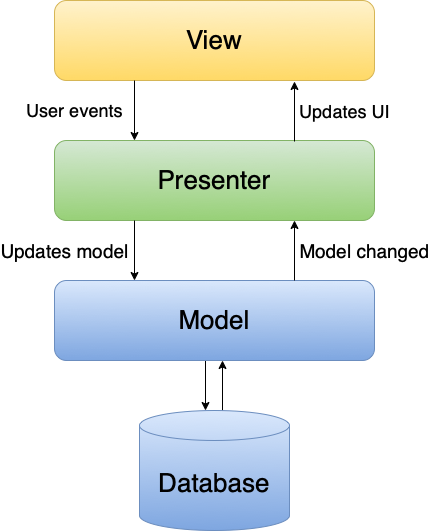
\includegraphics[scale=0.52]{../png/mvp_monolithic.png}
\caption{Monolithic architecture, MVP pattern}\label{picture:mvp}
\end{figure}

\noindent This architecture's main concept is having one code base that benefits in \\ simplifying development, testing, debugging, and deployment. \\
However, we can have those benefits only until the application grows large. Then all those processes get slower, more complex, and become problematic. In addition, with a lack of flexibility and scalability, it becomes challenging to maintain the application and keep it secure. \\

\noindent The BI-DBS portal is being developed by students. Students generally do not have much experience developing large applications and dealing with complex dependencies. Besides, they have limited time to progress in learning and developing the portal. Therefore it takes a lot of time for students to learn before contributing to the project. Thus it is more challenging to keep the application maintainable and ... (just one more example)


%%%%%%%%%%%%%%%%%%%%%%%%%%%%%%%%%%%%%%%%%%%%%%%%%%%%%%%%%%%%%%%%


\subsection{Technologies}
\paragraph*{PHP.} PHP is a general-purpose, open-source scripting language that can be integrated into HTML. It differs from client-side scripting languages in that its HTML is generated on a server and then sent to a client. That feature allows rapidly building a web application with a thick server and thin client. This is one of the approaches to using PHP to build an application, and it is used in the current project. \\
Using his approach leads to creating dependencies between the user interface and the application logic, that make any changes more effortful since a developer needs to adjust it on the both sides.

\paragraph*{Doctrine.} "Doctrine ORM is an object-relational mapper for PHP 7.1+ that provides transparent persistence for PHP objects. It sits on top of a powerful database abstraction layer. One of its key features is the option to write database queries in a proprietary object-oriented SQL dialect called Doctrine Query Language."\\ 
This framework did not cause any problems during the development process and does not have any valuable disadvantages for the BI-DBS to operate properly.

\paragraph*{Nette.} Nette is an open-source framework for creating web applications in PHP. It helps with developing both the client and server sides of the application and also reduces security vulnerabilities.\\ 
Frontend and backend dependencies are strengthened, indicating that they are a single unit. The fact that the they are so strongly dependent is a drawback. Because of this, it is difficult to make changes to one side without having an impact on the other.

\paragraph*{Latte.} Nette framework uses a template system Latte. It compiles templates down to the optimal PHP code.

\paragraph*{AdminLTE.} AdminLTE is a fully responsive administration template. Based on Bootstrap 4.6 framework and also the JS/jQuery plugin. 

\paragraph*{Vue 2.} Vue.js is a javascript framework for building user interfaces and single-page applications.\\
Most of the frontend is implemented using Latte templates and AdminLTE bootstrap. However, in order to reduce dependencies between the frontend and the backend, and also modernize it, few components were refactored to the Vue.js version 2. The logic is defined using the Options API. It is traditional object-oriented way, and up until Vue 2 it was the only way to create components in Vue.

\paragraph*{Javascript.} JavaScript is high-level programming language used for defining the behavior of webpages. It is a dynamically-typed scripting language that enables you to control multimedia, animate graphics, and generate dynamically changing content.\\ 
In the current BI-DBS portal it is used for defining logic on the frontend. Dynamically-typed languages are easy for development, but this feature reduces the code's readability, require more testing and are prone to run-time errors. Large applications like BI-DBS are likely to experience problems as a result of its drawbacks because it is better suited for smaller applications with simple logic.

%%%%%%%%%%%%%%%%%%%%%%%%%%%%%%%%%%%%%%%%%%%%%%%%%%%%%%%%%%%%%%%%

%%%%%%%%%%%%%%%%%%%%%%%%%%%%%%%%%%%%%%%%%%%%%%%%%%%%%%%%%%%%%%%%

\section{Planned state of the application} The main reason of creating a new application instead of refactoring the current one is a change of the application's architecture. A new modernized architectural design of the BI-DBS portal was composed by Ing. Andrii Plyskach in his master thesis\cite{mt-plyskach}. We are aiming to correct all the mistakes made in the current application. It is essential to ascertain that we have chosen the right stack of technologies according to the newly chosen architecture.

\subsection{Architecture}
Microservices architectural pattern\cite{architecture-haris} is based on the concept of a series of loosely-coupled services. They can be developed using different technologies and deployed independently. It is more complex architecture than a standard monolithic one. You can see the diagram illustrating microservices architecture in figure 1.2. 

\begin{figure}[hp]
\centering
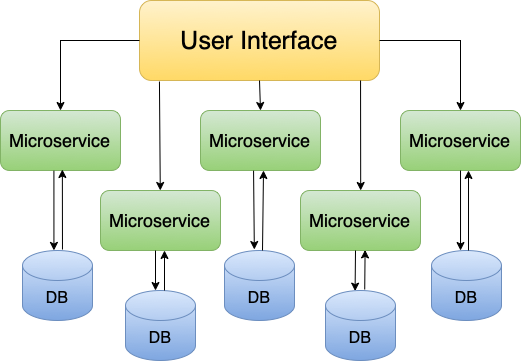
\includegraphics[scale=0.67]{../png/microservices.png}
\caption{Microservice architecture}\label{picture:mvp}
\end{figure}


\paragraph*{Advantages:}
\begin{itemize}
  \item \emph{Code readability:} When services are not strongly dependent the code appears to be better structured and easier for understanding and that is the crustal benefit for the BI-DBS portal.
  
  \item \emph{Independency in choosing a stack of technologies:} Microservices can be developed using different technologies which can be chosen according to the each microservice functionallity without affecting other microservices.
  
  \item \emph{Faster deployments:} Since all microservices can be deployed independently the deploying part is much smaller and the time for deploying one service is rather shorter.

  \item \emph{Fault tolerance:} Because of loose-coupling failing one of the microservices will not bring down the entire application.
\end{itemize}

\paragraph*{Disadvantages:}
\begin{itemize}
  \item \emph{Difficult debugging and testing:} Each service needs to be first tested separately and only then as one unit. Besides it is more difficult to track down errors.

  \item \emph{DevOps required:} To benefit from the fast deployment it should be configured and maintained. It requires the knowledge of development operations.

  \item \emph{Longer development time and limited reuse of code:} Microservices need to be managed separately, therefore it requires more time.
\end{itemize}

%%%%%%%%%%%%%%%%%%%%%%%%%%%%%%%%%%%%%%%%%%%%%%%%%%%%%%%%%%%%%%%%%%%%%%%


\subsection{Technologies}

\paragraph*{PHP.} Since version 5.0, PHP supports object-oriented functionality\cite{php-oop}. PHP is easy to learn, flexible, and supports all required functionalities for our application. It is used in a new project for a domain and business logic on the backend for API implementation.

\paragraph*{Symfony.} Symfony is a powerful back-end framework for creating complex applications which consists of reusable components.\cite{symphony-doc} Thanks to Doctrine Symfony provides all of the tools required to use databases in the application. It is constantly growing and improving, besides it has a strong community. It is easy to learn and has well-written documentation.


\paragraph*{Vue 3.} When the decision to create a new BI-DBS portal has not yet been made its frontend was getting modernized by rewriting components to Vue.js version 2. In the new project, it was chosen to carry on using the Vue.js framework but use a new version 3. This version comes with certain advantages for the application.\cite{vue3-updates}

\paragraph*{New features:}
\begin{itemize}
  \item \emph{Composition API:} Composition API is a set of APIs that allow us to create Vue components by importing functions rather than defining options. Mainly it benefits our project better code organization thus makes a project better structured and code easier to read. Moreover, Composition API enables efficient logic reuse.\cite{compositionapi-doc}
  
   \item \emph{Vite:} Vite is fontend build tool from the cratetor of Vue.js - Evan You. It is module bundler which is built on top of webpack, it will bundle the entire project on startup, hot reloads, and compilation. The primary purpose for the change is for speed. The server starts instantly since it uses native browser support for JavaScript modules.\cite{vite-doc}

   \item \emph{Increased rendering performance.}

\end{itemize}

\paragraph*{Typescript} Typescript is based on JavaScript which is dynamically typed. TypeScript has an additional syntax that makes it statically typed. That has advantages in catching errors during development. It also gives a code more structure and makes it predictable. Typescript is more suitable for big applications than JavaScript. For our project, it is crucial to write code that will be easy to read.\cite{typescript-doc}

\paragraph*{Quasar} Quasar is a web framework based on Vue.js. It provides us with ready-to-use components which are customizable and easy-extendable. Moreover, it makes the application less vulnerable to XSS attacks due to its escaping feature. When using Quasar, developers do not need deep knowledge of CSS and scripting languages to build a good-looking  and responsive application. Besides, it is suitable for developing single-page applications(SPA).\cite{quasar-doc}

\paragraph*{Pinia} Pinia is a Vue.js storage library and state management framework. It is mainly designed for the development of front-end web applications, and it uses declarative syntax as well as its own state management API.\cite{pinia-wiki}

%%%%%%%%%%%%%%%%%%%%%%%%%%%%%%%%%%%%%%%%%%%%%%%%%%%%%%%%%%%%%%%%

%%%%%%%%%%%%%%%%%%%%%%%%%%%%%%%%%%%%%%%%%%%%%%%%%%%%%%%%%%%%%%%%

\section{Summary and implications} The BI-DBS development team aims to dispose of problems and modernize the current project in every single aspect of development. Starting from choosing the right stack of technologies and designing a suitable architecture to implementing more complex and valuable features. However, even correctly chosen technologies and architecture for reducing the problems of the current project do not save us from the potential new challenges brought by the changes. 


\subsection{Summary} 
In order to summarize all changes and provide a better visualization of them, I arranged them all in Table \ref{demo-table}.\\
Evidently, the Nette framework is the core of the current project, which is responsible for managing the application in many ways. Although it can function well, it creates dependencies between the functionalities and makes the project less flexible, which is a significant disadvantage for large applications like the BI-DBS portal.\\
The planned state does not have dominating technologies that would cause this problem. Most of them are replaceable and flexible.





\begin{table}[ht]
\begin{tabular}{l|c|c|}
\textbf{}                                            & \textbf{Current state} & \textbf{Planned state} \\ \hline
\multicolumn{1}{|l|}{Architecture}                   & Monolitic              & Microservices          \\ \hline
\multicolumn{1}{|l|}{Backend language}               & PHP 7.2                & PHP 8.0                \\ \hline
\multicolumn{1}{|l|}{Backend framework}              & Nette                  & Symfony                \\ \hline
\multicolumn{1}{|l|}{Frontend framework}             & Nette, Vue.js 2        & Vue.js 3               \\ \hline
\multicolumn{1}{|l|}{Frontend templates and styling} & Latte, AdminLTE        & Quasar                 \\ \hline
\multicolumn{1}{|l|}{Scripting language}             & Javascript             & Typescript             \\ \hline
\multicolumn{1}{|l|}{Frontend templates and styling} & Latte, AdminLTE        & Quasar                 \\ \hline
\multicolumn{1}{|l|}{Module bundler}                 & Webpack                & Vite                   \\ \hline
\multicolumn{1}{|l|}{State management}               & Nette Sessions         & Pinia                  \\ \hline
\multicolumn{1}{|l|}{Routing}                        & Nette Router           & Vue.js Router          \\ \hline
\end{tabular}
\caption{\label{demo-table}Visualisation of changes.}
\end{table}

\subsection{Implications} From the analyses in sections \ref{sec12} and \ref{sec13}, we can see that existing problems in the current project are eliminated by chosen architecture and technologies for the planned state. Let's examine the main possible negative effects of the changes and how to deal with them.

\begin{itemize}
    \item Microservices architecture provides such advantages as agility and fast deployment. This architecture is more complex in comparison with a monolithic one. Therefore it comes along with establishing some of the DevOps principles for the project. Mainly configuring continuous integration and automated deployment. DevOps concepts and automation including CI and CD are described in the chapter \ref{chap2}.
    \item In the current application, Nette is a core full-stack framework that is also responsible for managing the application's security. Besides, the monolithic architecture allows you to store all the data on the server side. The communication between the client side and server side is secure.\\
    In microservices applications, there is constant communication between the frontend and the backend and exchanging sensitive data. Therefore it is crucial to control every step of that communication with control of permissions and inputs validation on both the client and server sides. Thus the application should have a clearly defined access management system which I will introduce in the chapter \ref{chap3}.
    \item Since all the services are developed, deployed and tested separately, there is a higher chance of failure in communication between them. Obviously, It is not enough to test only the functionalities of singles services but to test their integration. Therefore it is essential to design a new integration testing system for the application. It is necessary to eliminate the possibility of the cascade failure of services.
\end{itemize}


%%%%%%%%%%%%%%%%%%%%%%%%%%%%%%%%%%%%%%%%%%%%%%%%%%%%%%%%%%%%%%%%

\chapter{Analysis of the DevOps model} The DevOps and microservices are two important trends in application development. Considering that both of them are mainly focused on providing better agility, flexibility, and operational efficiency, we can assume that they would work better together. \cite{devops-micr}\\ 
In this chapter, I will describe the main DevOps concepts and practices, analyze their possible advantages for the BI-DBS application and decide whether adopting the DevOps model would be beneficial. 

%%%%%%%%%%%%%%%%%%%%%%%%%%%%%%%%%%%%%%%%%%%%%%%%%%%%%%%%%%%%%%%%

\section{What is DevOps?} The term \textbf{DevOps} is derived from the combination of software \textbf{dev}elopment and IT \textbf{op}eration\textbf{s}.\\
DevOps is a relatively new term. Around 2007 and 2008 concerns about the separate work of software creators and software operators were raised. The concept started to grow on online forums and meet-ups. The first conference named "DevOps" was held in 2009.\cite{devops-wiki}\\
DevOps is a software development methodology composed of a set of cultural philosophies, practices, and tools that improve an organization's ability to deliver applications, services, and improve products faster than traditional software development and infrastructure management processes. It represents a cultural shift that has a significant effect on a team that adopted that methodology and the software they make.\cite{devops-atl}




%%%%%%%%%%%%%%%%%%%%%%%%%%%%%%%%%%%%%%%%%%%%%%%%%%%%%%%%%%%%%%%%

\section{DevOps concepts} DevOps concepts are a common set of rules which are the core of this methodology. It is not just tools, but a cultural philosophy, a way of project life-cycle organization. 

\subsection{Constant Improvement} Constant improvement is a special concept and practice of DevOps methodology. The main idea is a focus on improvements, updates, and experimenting. It tells each team member not to be afraid of failures but take them as an opportunity to learn, whatever the outcome of an experiment, a person will have a deeper understanding of what works and what does not. Besides this rule gives more responsibility to a person and allows them to consistently push code changes to minimize waste, do speed optimization and improve development efficiency.


\subsection{Collaboration} The term DevOps itself is a collaboration of two words as well as one of its concepts is a collaboration of different IT departments. That means that the roles in the team are not so strict and independent as in a traditional work and team organization. Developer and IT operations roles are getting closer to full-stack roles. Leading to a better understanding of the software development life-cycle by the whole team.\\
It goes great together with the microservices architecture which is, by the way, becoming a standard for DevOps. A developer does not have the main focus on understanding the logic of the application because it's simplified by the architecture but instead is more focused on technological and operational processes. 

\subsection{Automation} DevOps approach is meant to benefit in fast development and improvement. Needless to mention that automation is one of the golden rules for increasing the speed of the application life-cycle. Everyone should aim to automate as many phases of the process as it is possible. As a result team members are satisfied with a decreased need for doing repetitive tasks. Thus they can focus on significant tasks and work on new features. Overall it helps minimize human errors and boosts team output. Automation is a key element of a CI/CD pipeline, more about CI/CD in section 2.3.

\subsection{Data-Based Decision Making} With the DevOps approach decisions from choosing a technology stack for the application to adding features should be made based on collected data. The first part should be always collecting as much relevant data as it is possible. Then, based on the collected data analysis of the team, a decision should be made. It helps to create software that solves real problems effectively. Decisions made without considering client feedback data, colleagues' opinions, and proper analysis would lead to creating badly-functional software full of useless features which does not fulfill the client's needs.

\subsection{Responsibility Throughout the Lifecycle} DevOps methodology comes with a requirement for team members to fully understand the process of software development from the feature idea to implementation and deployment and take responsibility for it.\\
End-to-end responsibility helps to reduce failures and resolve bugs quickly.
% When all team members are aware of the 












%%%%%%%%%%%%%%%%%%%%%%%%%%%%%%%%%%%%%%%%%%%%%%%%%%%%%%%%%%%%%%%%

\section{DevOps cycle and practices} DevOps concepts reflect in a set of practices during the DevOps delivery cycle. The cycle is visualized in Figure 2.1. These practices mainly represent the automation concept but also come together with other concepts.\cite{devops-principles}

\begin{figure}[h]
\centering
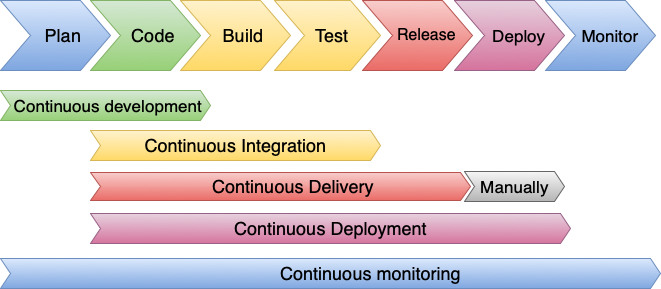
\includegraphics[scale=0.56]{../png/devops.png}
\caption{Devops cycle and practices}\label{picture:devops}
\end{figure}

\subsection{Continuous development} Continuous development is a practice composed of agile planning and coding. The goal of agile planning  is to divide big problems into smaller logical problems, estimate the complexity of created tasks and plan the amount of tasks for some short time period(sprint), usually it is from one to four weeks period. This method allows getting some large significant tasks done in a shorter time, because after its division developers can work on the subtasks simultaneously and it is more effortless for testing.

\subsection{Continuous integration (CI)} In order to avoid a problem with the integration of large parts of code, DevOps CI offers continuous pushing the code changes to the remote shared repository on the server. Every change pushed to the repository triggers a build and tests configured in a CI pipeline to make sure new changes do not affect already functioning features and also does not contain new errors.

\subsection{Continuous delivery (CD)} Continuous delivery is an extension of continuous integration. After building and testing the code from the repository it automatically deploys releases to the testing environment and also prepares it to be deployed to the production. It requires human intervention to deploy a release to production. This is a safer version of fast and frequent deployment, in a case when the pipeline does not contain strong testing tools and the application needs to be tested manually.

\subsection{Continuous deployment (CDE)} Coupled with continuous delivery, the continuous deployment also deploys the release to the production. Using this practice no human intervention is required. Every change pushed to the main shared remote repository will be automatically deployed to production. The only obstacle to the deployment would be a failed build or test.

\subsection{Continuous monitoring (CM)} Continuous monitoring is an automated method that allows to observe and discover compliance concerns and security vulnerabilities throughout the DevOps lifecycle. It also finalizes the cycle by providing feedback on monitoring and informing about existing or possible failures. It helps to resolve issues in real-time.

\subsection{Infrastructure as Code (IaC)} Infrastructure as a code is a practice of managing infrastructure that enables automation in the DevOps lifecycle. It offers using scripts for configuring deployment environment and other infrastructure, including establishing a version control system.

\subsection{Containerization} Containerization is the practice of packaging an application in one container. It provides better flexibility for deployment and needs fewer resources to run. Currently, Docker provides the most frequently used container toolset.
% https://www.docker.com


%%%%%%%%%%%%%%%%%%%%%%%%%%%%%%%%%%%%%%%%%%%%%%%%%%%%%%%%%%%%%%%%

\section{DevOps adoption}\label{devops:adp} The idea of adopting the DevOps model came to me with a need to configure the new deployment of the new BI-DBS portal due to the transfer to microservices architecture. Before analyzing the DevOps concepts, I assumed that the DevOps model is just an automation idea. In fact, I was wrong and did not know it is a solid methodology bringing huge advantages to the project. From my own observations, it is a pretty common misunderstanding of the DevOps model, which leads to missing out important concepts.\\ 

\noindent "Even while automation helps speed up manual operations, cooperation and communication are the key objectives of DevOps. Automating your operations won’t bring about the desired business benefits unless everyone involved in the software development, delivery, testing, and operating processes adopts excellent communication and collaborative practices." \cite{devops-adoption}\\
The analysis makes it clear that the DevOps model is suitable and valuable for the BI-DBS portal project management and development.

\paragraph*{Adoption steps:} 


\begin{enumerate}
    \item \emph{Devops philosophy.} This thesis can be used to introduce the DevOps methodology to students. Before getting to development as well as learning the processes of development students should learn team organization management including DevOps concepts. 
    \item \emph{DevOps Practices.} Analyze which practice we would like to adopt and how it will be beneficial and then complete the three next steps:
        \begin{enumerate}
            \item Choosing relevant tools for a practice we would like to adopt
            \item Application of the practice using chosen tools
            \item Document the configuration of the practice for a team
        \end{enumerate}
    I will adopt the most important DevOps practices for the BI-DBS portal in the chapter \ref{chap5} using these steps.
\end{enumerate}




%%%%%%%%%%%%%%%%%%%%%%%%%%%%%%%%%%%%%%%%%%%%%%%%%%%%%%%%%%%%%%%%


\chapter{Access management}
8 role -> 3 role
aktory, diagramy pristupu do modulu a component (zhruba) konkretni implementace je na tom kdo dela navrh modulu

\chapter{Implementation}
\chapter{Automation}
\chapter{Testing}





% {Design and implementation of Authentication \& Authorization}

% The BI-DBS portal transfers to microservices architecture and gets \\  
%  modernized. In order to keep the application secure, a new identity and access management must be designed. In this chapter, I will describe the design for implementation of Authorization and Authorization, including the user roles and permissions management.

%%%%%%%%%%%%%%%%%%%%%%%%%%%%%%%%%%%%%%%%%%%%%%%%%%%%%%%%%%%%%%%%

% \input{tex/3.1_Authetication}

%%%%%%%%%%%%%%%%%%%%%%%%%%%%%%%%%%%%%%%%%%%%%%%%%%%%%%%%%%%%%%%%


% \section{Authorization}\label{sec:authorization}

% \subsection{Roles}

% \subsection{Permissions}

% \section{Implementation}

% \section{Tests}







\chapter{Automation -- CI/CD}

%%%%%%%%%%%%%%%%%%%%%%%%%%%%%%%%%%%%%%%%%%%%%%%%%%%%%%%%%%%%%%%%

\section{Used tools}\label{sec51} First step of adopting the automation concept is choosing suitable tools for the planned automation of processes.


\subsection{Docker} Docker is an open-source platform that allows to build, run and deploy applications quickly using virtualization of server hardware in containers. Containers are lightweight units created by the containerization of the application. The containerization provided by Docker is a technology of software packaging including code, libraries and other necessary dependencies and configurations for building the application.\\
Docker was already chosen as a tool for running the application and I have decided to also use it for the automation of building and development processes due to its flexibility, lightweight containers and speed. \cite{docker, docker-2}

\subsection{GitLab} GitLab is a web service based on the Git version control system that is also a DevSecOps \cite{devsecops} platform with multiple functionalities. It allows to plan, track and manage issues, as well as manage automation processes using CI/CD pipelines. Besides it lets to schedule jobs, create merge requests, do code reviews and provides many other features. Its main benefit is that a software development team can use GitLab instead of using many other tools as it combines many features. \cite{gitlab, gitlab-2}\\
GitLab is generally used for many school applications including the BI-DBS portal. Therefore it was the obvious choice to use it for the automation processes. 



\subsection{CloudFIT} CloudFIT is a platform for everyone from FIT CTU, which provides server management from usual web applications hosting to complex calculations and simulations. \cite{cloudfit}\\
I have chosen CloudFIT for hosting the BI-DBS frontend, because the servers are managed by the faculty and faculty workers are open to consulting the server parameters. Besides, it is free of charge, has well-written documentation and is recommended for hosting school applications.

\subsection{Buildah} Buildah is a tool for containerization which is compatible with for example Docker. I have decided to use Buildah because the faculty provided an image with Buildah for building docker containers, which is ready to use. Besides, from my own small research comparing it with for instance Docker in Docker(dind) it turned out to be the most stable and efficient variant. \cite{buildah}


\subsection{Nginx} Nginx is an open-source web server that can run in a docker container and allows numerous configuration options such as reverse proxy, load balancing, caching and others. The decision to use Nginx was made due to its simplicity in configuration. \cite{nginx, nginx-2}


\subsection{Yarn} Yet Another Resource Negotiator(Yarn) is a JavaScript package manager which helps to manage project dependencies. It assists the application with managing packages, managing scripts and caching. Yarn was already in use in the BI-DBS frontend project, it has valuable benefits over other package managers like for instance parallel installation of packages and installation of packages without an internet connection. \cite{yarn, yarn-2}


%%%%%%%%%%%%%%%%%%%%%%%%%%%%%%%%%%%%%%%%%%%%%%%%%%%%%%%%%%%%%%%%

\section{Implementation} Second step of adopting the automation practices is setting up the processes using chosen tools. The implementation goal is to pro


\subsection{Containerization}  I have adopted the containerization using Docker for a use in CI/CD pipeline. The Dockerfile simply contains the instruction for building a Docker images. It composed of specific commands which tell how to build the image. A Docker image is a read-only file containing a set of instructions. When these instructions are executed, a Docker container is created. 
%https://www.simplilearn.com/tutorials/docker-tutorial/what-is-dockerfile


\begin{lstlisting}[language=Octave, caption=Dockerfile]
FROM node:latest as build
WORKDIR /app
COPY package*.json ./
RUN yarn
COPY ./ .
RUN yarn run build

FROM nginx
RUN mkdir /app
COPY --from=build /app/dist /app
COPY nginx.conf /etc/nginx/nginx.conf
\end{lstlisting}

\noindent Dockefile showed on listing 5.1 contains installing dependencies on the fifth row and application bundling on the six's row using Yarn and also adding Nginx configuration from the \texttt{nginx.conf} file on the last row, which defines parameters like hostname, listen port and others.



\subsection{CI/CD pipeline configuration} CI/CD pipeline is a set of steps that are executed when the pipeline was triggered.\\
Listing 5.2 shows all the stages of the CI/CD pipeline. First two stages where configured by Ing. Oldřich Malec with the first setup of the frontend projects. Download stage installs all the dependencies required for the application run. Codestyle stage provides linting of the source code. Other three stages I have implemented in this thesis.
\begin{lstlisting}[language=Octave, caption=Gitlab CI/CD stages]
stages:
  - download
  - codestyle
  - test
  - build
  - deploy
\end{lstlisting}

\noindent GitLab provides the visualization of the pipeline steps and allows to execute any steps manually as well as monitor the log of any job from the pipeline. Figure 5.1 shows how the passed pipeline looks in the BI-DBS portal frontend.

\begin{figure}[ht]
\centering
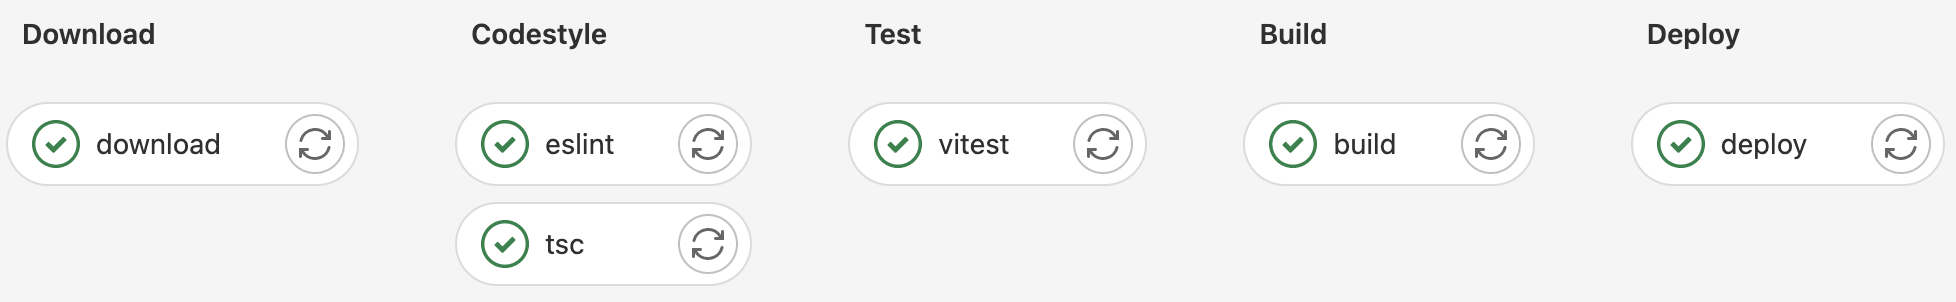
\includegraphics[scale=0.377]{../png/pipeline.png}
\caption{CI/CD pipeline in GitLab}
\end{figure}

\noindent The pipeline stages are executed from left to right and if any of the stages fails all the other ones will be skipped. It helps to avoid pointless running of jobs, because the stages are put in the way that they depend on the result of the previous ones. 




\subsubsection{Test} Test stages contains one job which I have named vitest, because it executes unit tests implemented using Vitest framework which will be introduced in the six's chapter. For running the tests I have used Yarn, which provides the tests execution by running just one command which is added to script section on the line fifteen of the listing 5.3. 
\begin{lstlisting}[language=Octave, caption=Test stage in the CI/CD pipeline]
.image_template: &image
  image: $CI_REGISTRY/ict/images/alpine/ci:3.16
  before_script:
    - apk add -U nodejs yarn

.cache_pull_template: &cache
  key: $CI_COMMIT_REF_SLUG
  paths:
    - node_modules/
    
vitest:
  <<: *image
  stage: test
  script:
    - yarn run test
  cache:
    <<: *cache

\end{lstlisting}

\noindent For the tests execution setup in the pipeline I have used image and cache pull templates, which were already prepared and used for the download and codestyle stages.




\subsubsection{Build} Build stage is focused on building an image and adding it to the GitLab container registry of the project. I have used the faculties image containing buildah and buildah itself for the script which is shown in listing 5.4. Command from the row number seven will create the image and the next command from the row number eight will upload it to GitLab registry.\\

\begin{lstlisting}[language=Octave, caption=Build stage in the CI/CD pipeline]
build:
  image: $CI_REGISTRY/ict/images/buildah:v1
  stage: build
  variables:
    IMAGE_TAG: $CI_REGISTRY_IMAGE:$CI_COMMIT_REF_NAME
  script:
    - buildah build --squash --tag $IMAGE_TAG -f Dockerfile
    - buildah push $IMAGE_TAG
  only:
    - devtest
\end{lstlisting}

\noindent The last two rows of the listing define the only branch for which this job will be executed. The BI-DBS frontend does not have a production version yet. Therefore I have decided to create the environment for deploying the application for testing during the development process. For that reason I have created a branch named devtest, any changes pushed to which will be automatically built and deployed.


\subsubsection{Deploy} When it comes to deploy stage, it means that the application when though all the previous pipeline stages and application is ready to be deployed. The deployment process of the CI/CD pipeline is composed of execution of deployment script from the server. For the connetion to the server GitLab uses CI/CD variable which allow securely storing sensetive data, which need to be used in the pipeline like for example deployment user showed on line number six of listing 5.5.


\begin{lstlisting}[language=Octave, caption=Deploy stage in the CI/CD pipeline]
deploy:
  stage: deploy
  dependencies:
    - build
  script:
    - ssh -A "${DEPLOYER_IP_ADDRESS}" -l ${DEPLOYER_USER} 'bash deploy-dbs-frontend.sh'
  only:
    - devtest
\end{lstlisting}


\noindent Deployment script contains few steps such as pulling Docker image from the GitLab created in the build stage, then creating and running a container and logging the container running. The configuration of this process is securely stored on the server.

%%%%%%%%%%%%%%%%%%%%%%%%%%%%%%%%%%%%%%%%%%%%%%%%%%%%%%%%%%%%%%%%

\section{documentation}

%%%%%%%%%%%%%%%%%%%%%%%%%%%%%%%%%%%%%%%%%%%%%%%%%%%%%%%%%%%%%%%%
\chapter{Testing} I have provided two types of tests. First of them is unit tests, created specially for the CI pipeline, which tests the main functionalities like managing the data and processing of authentication and  authorization processes. Second type of tests is manual functional tests. I have created test scenarios for manuals testing of all the implemented features, including the cases for different roles.

%%%%%%%%%%%%%%%%%%%%%%%%%%%%%%%%%%%%%%%%%%%%%%%%%%%%%%%%%%%%%%%%

\section{Tests for CI} Providing a set of regression tests for the CI pipeline is clearly good practice, since they will be executed with every change provided to the remote repository and make sure that if any of those changes will affect the functionality of the tested code the pipeline will fail and the code with defects will not be deployed. Moreover, tests will tell the developer exactly what unit was affected by their changes and require a fix.


\subsection{Vitest} Vite is a frontend build tool used for the BI-DBS frontend. Vitest is a unit test framework built on top of Vite. It is a suitable tool for implementing tests in the project like the BI-DBS frontend which uses Vite. Vitest cares a lot about performance and speed, which makes it a good choice for tests that will be a part of CI pipeline. \cite{vitest}

\subsection{Tests} The authorization module is composed of four main services which I have implemented for authentication and authorization processes including additional features like a refreshing of token and logging out. Therefore I have created unit tests for the functionalities of those services.\\


\paragraph*{Generating the access token service.} The process of getting the access token enables the application to log in the user on the frontend after an authorization server has successfully authorized the user and provided the client with the authorization code. This service is focused on exchanging that code for an access token with the backend and handling the response from the server.


\paragraph*{Test cases for the token generating service} 
\begin{itemize}
    \item \emph{Positive scenario:} 
        \begin{itemize}
            \item \emph{Conditions:} A valid token is successfully returned in the valid response.
            \item \emph{Expected result:} User was successfully authorized.
        \end{itemize}
    \item \emph{Negative scenario} 
        \begin{itemize}
            \item \emph{Conditions:} An invalid token is successfully returned in the valid response.
            \item \emph{Expected result.} The errors from parsing the token are successfully handled and the user was not authorized.
        \end{itemize}
    \item \emph{Negative scenario.} 
        \begin{itemize}
            \item \emph{Conditions:} The request for getting the access token fails.
            \item \emph{Expected result:} The errors from the request are successfully handled and the user was not authorized.
        \end{itemize}
\end{itemize}

\

\paragraph*{Refreshing the access token service.} Refreshing process prolongs the authorized status for a user without the need of submitting credentials, which is implemented by exchanging the refresh token and current access token for the new access token with the backend. 


\paragraph*{Test cases for the token refreshing service} 
\begin{itemize}
    \item \emph{Positive scenario:} 
        \begin{itemize}
            \item \emph{Conditions:} User is authorized and the request for refreshing the access token succeeded and the server returned a new valid access token.
            \item \emph{Expected result:} The authorization time for a user was prolonged to the expiration time of the newly received access token.
        \end{itemize}
    \item \emph{Negative scenario} 
        \begin{itemize}
            \item \emph{Conditions:} User is authorized and the request for refreshing the access token succeeded but returned an invalid token.
            \item \emph{Expected result.} The errors from parsing the token are successfully handled and the user was logged out.
        \end{itemize}
    \item \emph{Negative scenario.} 
        \begin{itemize}
            \item \emph{Conditions:} The request for refreshing the access token fails.
            \item \emph{Expected result:} The errors from the request are successfully handled and the user was not logged out.
        \end{itemize}
\end{itemize}

\


\paragraph*{Rejecting the access token.}The process of logging out is implemented as a rejection of a token which includes removing all of the user's data from the user's store along with permissions to access the components which require authorization.

\paragraph*{Test cases for the token rejecting service} 
\begin{itemize}
    \item \emph{Positive scenario:} 
        \begin{itemize}
            \item \emph{Conditions:} User is authorized and the request for rejecting the access token succeeded.
            \item \emph{Expected result:} User was successfully logged out.
        \end{itemize}
    \item \emph{Negative scenario} 
        \begin{itemize}
            \item \emph{Conditions:} The request for rejecting the access token fails.
            \item \emph{Expected result.} The errors from the request are successfully handled and the user was logged out.
        \end{itemize}
\end{itemize}


\


\paragraph*{Authorization service.} The services described above also need some additional functionalities like parsing the data from the request and preparing the URL for communication with the authorization server which are implemented in the authorization service with both positive and negative scenarios. 


\paragraph*{Test cases for the authorization service} 
\begin{itemize}
    \item \emph{Positive scenario:} 
        \begin{itemize}
            \item \emph{Conditions:} The frontend calls the function to create an URL to initiate an authorization process by sending a request to the authorization server,
            \item \emph{Expected result:} The URL is valid.
        \end{itemize}
    \item \emph{Positive scenario.} This scenario is used for the implementation of four tests for each user's role: admin, guarantor, teacher and student
        \begin{itemize}
            \item \emph{Conditions:} The frontend calls the function to process the access JWT token it got from the server for authorization of a user with a certain role.
            \item \emph{Expected result.} Successfully parsed the token and the data in the user store matches the user's identity sent in a token including the role.
        \end{itemize}
\end{itemize}

\ 

\paragraph*{The results of unit testing.} Frankly speaking, in the beginning I have underestimated the importance of the unit tests implementation as I was very confident about my code as it was structured and clear for me to work correctly. Moreover, multiple times I have successfully tested all the functionalities manually myself.\\
Unexpectedly, The implementation of the unit tests process helped me to uncover and correct some weaknesses in the implementation of some functions. But most importantly, thanks to the creation of tests with also negative scenarios I have found some unhandled errors and was able to test the implementation in the various conditions.\\
The full set of tests is added to the CI pipeline and executed by every change pushed to the repository. The duration of tests as you can see in Figure 6.1 is less than four seconds, which is a remarkably good result.

 \

\begin{figure}[h]
\centering
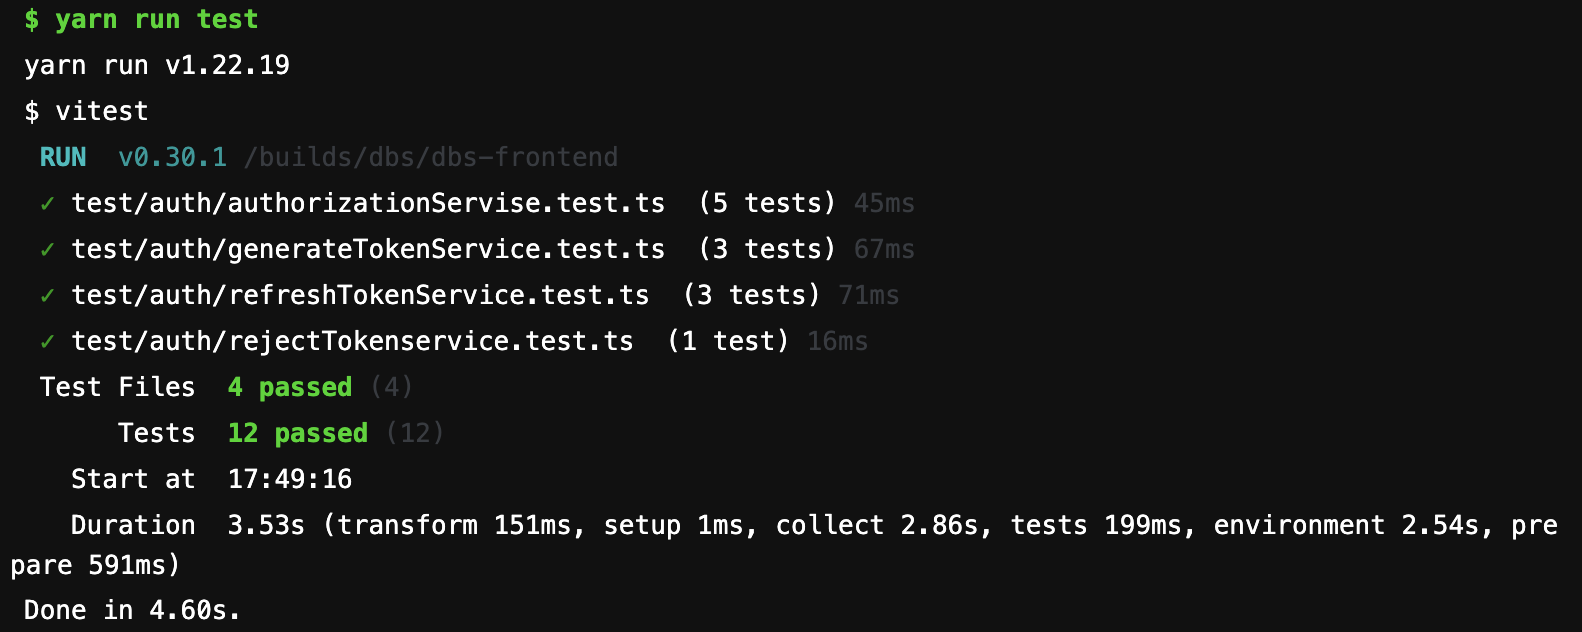
\includegraphics[scale=0.47]{../png/tests.png}
\caption{CI tests}\label{picture:tests}
\end{figure}


%%%%%%%%%%%%%%%%%%%%%%%%%%%%%%%%%%%%%%%%%%%%%%%%%%%%%%%%%%%%%%%%

\section{Manual testing} I have prepared a scenario for manual testing of all implemented features by the developers and also the group of users of the application. 

\paragraph*{Roles.} The test must be provided for each of the roles separately. \\
The roles are admin, guarantor, teacher, and student.

\paragraph*{Conditions.} 
\begin{itemize}
    \item  Client and Server applications are running.
    \item  Semester import was made, the user's username exists in the database and has at least one role for the imported course.
    \item  User must have access to the database of connections microservice to change the roles for tests.
    \item  The expiration time of the access token is mocked for 5 minutes.
\end{itemize}

\paragraph*{Test.} \

\begin{table}[h]
\begin{tabular}{|c|l|l|}
\hline
\multicolumn{1}{|l|}{} & Test Step:                                                                                                                                                           & Expected result:                                                                                                         \\ \hline
1.                     & \begin{tabular}[c]{@{}l@{}}Try to access the home\\ page of the application.\end{tabular}                                                                            & Redirection to the login page.                                                                                           \\ \hline
2.                     & Clicks on the login button.                                                                                                                                          & Redirected to the login form.                                                                                            \\ \hline
3.                     & \begin{tabular}[c]{@{}l@{}}Submitted login form with\\ valid credentials.\end{tabular}                                                                               & Redirected to the home page.                                                                                             \\ \hline
4.                     & \begin{tabular}[c]{@{}l@{}}Control all the displayed \\ navigation tabs to be \\ correct for your role.\end{tabular}                                                 & Tabs are displayed correctly.                                                                                            \\ \hline
5.                     & Refresh the page.                                                                                                                                                    & \begin{tabular}[c]{@{}l@{}}Page was successfully refreshed, \\ user still has access to the \\ application.\end{tabular} \\ \hline
6.                     & \begin{tabular}[c]{@{}l@{}}Leave a browser page with an\\ application open for 5 minutes\\ and then click to one of the tabs \\ from the navigation bar\end{tabular} & \begin{tabular}[c]{@{}l@{}}Component loaded by the path\\ of navigation tab.\end{tabular}                                \\ \hline
7.                     & Click the logout button.                                                                                                                                             & \begin{tabular}[c]{@{}l@{}}The modal window displayed and \\ requires the submission to log out.\end{tabular}            \\ \hline
8.                     & Submit.                                                                                                                                                              & Redirected to the login page.                                                                                            \\ \hline
\end{tabular}
\end{table}

\paragraph*{Results.}


%%%%%%%%%%%%%%%%%%%%%%%%%%%%%%%%%%%%%%%%%%%%%%%%%%%%%%%%%%%%%%%%


\setsecnumdepth{part}
\chapter{Conclusion} First of the thesis goals was contributing to the project by improving the development efficiency and maintenance, which was achieved by introducing the DevOps methodology and also automating such processes as testing and development. The next goal was defined as adjusting the project to make it more structured and secure. Therefore, I have analyzed the current access management structure and came to the conclusion that it is unnecessarily too complicated. I have managed to logically simplify it and provide a design of a new access management system. Moreover, based on the clear permissions system I have strengthened the security by providing validation before every user's request. Finally, I planned to implement the authentication and authorization features. These functionalities were created using the OAuth 2.0 protocol and authorization microservice. Furthermore, I have reduced security vulnerabilities by providing a suitable way of storing sensitive data.\\
In my opinion, this thesis will definitely be useful for developers and managers of the BI-DBS portal. It can be used as a part of introduction materials to DevOps methodology for new students before getting to the application development as well as the documentation of the access management system for managers and developers.\\
From the analysis of the current and planned application state, I have outlined three challenges, which we are facing in the new application state due to the microservices architecture. I have provided the solutions for two of them. The deployment problem was resolved by automation of this process. Possible security vulnerabilities were decreased by creating an access management system. The testing challenge still remains unresolved. The application needs a strong set of integration tests. Ideally, they should be a part of CI/CD pipeline to reduce the probability of deploying errors. This is an idea for further improvement which can become a topic for a thesis or a set of tasks for the teams of BI-DBS developers.\\
Thanks to this thesis I have learned a lot about application security and efficient development. Moreover, from the development of the features I got experience working with modern technologies such as Vue.js, Typescipt, Pinia and others.

\printbibliography[title=Sources]

\setsecnumdepth{all}
\appendix
\chapter{Acronyms}
\begin{description}
    \item[BI-DBS] Database systems
    \item[BI-SP1] Team software project 1
    \item[BI-SP2] Team software project 2
    \item[CI] Continuous integration
    \item[CD] Continuous development
    \item[CSRF] Cross-site request forg
    \item[DevOps] Development and Operations
    \item[HTML] HyperText Markup Language
    \item[HTTP] HyperText Transfer Protocol
    \item[IT] Informational technology
    \item[JS] JavaScript
    \item[MVP] Model View Presenter
    \item[OAuth] Open authorization
    \item[ORM] Object Relational Mapping
    \item[PHP] Hypertext Preprocessor
    \item[SPA] Single-page application
    \item[SQL] Structured Query Language
    \item[URL] Uniform Resource Locator 
    \item[XSS] Cross-site scripting
\end{description}


\chapter{Contents of enclosed CD}

%change appropriately

% \begin{figure}
% 	\dirtree{%
% 		.1 readme.txt\DTcomment{the file with CD contents description}.
% 		.1 exe\DTcomment{the directory with executables}.
% 		.1 src\DTcomment{the directory of source codes}.
% 		.2 wbdcm\DTcomment{implementation sources}.
% 		.2 thesis\DTcomment{the directory of \LaTeX{} source codes of the thesis}.
% 		.1 text\DTcomment{the thesis text directory}.
% 		.2 thesis.pdf\DTcomment{the thesis text in PDF format}.
% 		.2 thesis.ps\DTcomment{the thesis text in PS format}.
% 	}
% \end{figure}

\end{document}